% main.tex, to be used with thesis.tex
% This contains the main work of your thesis.

%\bibliography{thesis}  % uses the references stored in Chapter1Radar.bib

\chapter{Data Persistence Technology for Sensor Networks: An Empirical-based
Choice for NetBEAMS}

This chapter analyzes each of the taxonomies defined in chapter
\ref{chap:taxonomies} against different other variables. First, the
requirements defined by NetBEAMS, as our case study in chapter
\ref{sec:problem-requirements}, is be compared. Then, the scope of this work is
compared to the technologies selected based on the readings of the
literature review in persistence in sensor networks and other new trends in
performance. Finally, a table summarizes the contenders strenths and discusses
the selected technology to be integrated with the design of a Data
Persistence component.

\section{Scope of the use of the Techonolgy}

The scope of the use of the database can cover different functional and
non-functional requirements defined in the previous chapter. This work does
not intend to implement an application based on the database system selected,
but provide the foundation of a database management system that can be used to
develop one focused in less refactoring and high scalability and performance.
For this reason, the use of the database system will be restricted to the data
persistence and use through native system or through the use of native
programming languages or API. In this way, the scope of this technology
selection is can be summarized as follows:

\begin{itemize}
  \item Provide data management over the collected sensor data, as a regular
  database system;
  \item Must be able to scale in the face of an increase to the data load of
  the sensor network, as described in chapter 2;
  \item Must be able to use single or multiple servers to improve performance
  and optionally deal with Data-Centric approaches to sensor data partitioning;
  \item Must provide a data model that scales, decreasing the constant data
  schema changes.
\end{itemize}

\section{Database Systems Contenders}

This section describes the database systems contenders considered to be used
together with for the implementation of the Data Persistence component for
NetBEAMS. As described in the previous chapter, the selection of the
technologies must be based on the list of functional and non-functional
requirements specified within the scope this work, defined in the previous
section.

One of the primary questions related to data persistence is regarding the data
model and type of the database, that is, the use of relational model or
structured models. In addition to that, and given the current time of academic
research and new trends distributed computing such as Cloud Computing and the
Internet \cite{cloud-comp-survey}, the selection of a data persistence for
sensor networks should maintain a wider spectrum of the types of database
systems. Among other intriguing questions, \cite{db-is-rdbs-dommed} reflects
about the use of alternatives to the relational model for dynamic environments
such as data persistence for the Web. Similarly, these trends are also related
to the advances of Cloud Computing and its persistence layer as a solution to
dynamic systems \cite{cloud-comp-architectures}. For this reason, this work
also included the overview of alternative data models for the development of
an experiment that brings data persistence to NetBEAMS. In such a fashion, the
list of the systems considered for evaluation is the following:

\begin{itemize}
  \item \textbf{MySQL}\cite{mysql}: an open-source relational database system
  that is the primary choice of the development of projects of different sizes. It was selected
  because of its popularity in the current community;
  \item \textbf{Oracle}\cite{oracle}: is the most popular commercial database
  system, having a campus wide academic licenses availabe;
  \item \textbf{TinyDB}\cite{tinydb}: as referred in the literature review,
  TinyDB is a database system used in many different sensor networks implementation
  \cite{sn-db-tinydb};
  \item \textbf{MongoDB}\cite{mongodb}: an open-source key-value database system
  described in the article that questions the use of the relational model
  \cite{db-is-rdbs-dommed}, as well as the Cloud Computing trends survey
  \cite{cloud-comp-architectures}.
  \item \textbf{DB2}\cite{db2}: in the search of an XML database system, DB2 is
  listed as a hybrid database system that offers both XML and relational model
  \cite{db-xml-enabled}. It was selected because NetBEAMS can represent the
  collected data in the XML format \ref{sec:dsp-message}.
\end{itemize}

These technologies will be reviewed in contrast to their capabilities to adhire
to the specifications of the taxonomies defined in chapter 3 and the
requirements and the scope for a data persistence of NetBEAMS, as defined in
chapter 4.

\section{Analysis of the Purpose of Sensor Data}

The execution of the SF-BEAMS sensor network, together with the NetBEAMS
automated infrastructure, can be summarized as follows:

\begin{itemize}
  \item Data is generated by sensor devices, such as the YSI sonde
  \cite{YSI-Sonde}, and manually collected by using a laptop to the network
  sink at the RTC laboratories;
  \item Upon data reception, the RTC staff index and archive the data for
  for distribution using the OPEnDAP format;
  \item An automated approach to the data collection procedures is done
  using NetBEAMS \cite{netbeams2009}, using software components to extract and
  send the data to the network sink. A complete description of this approach
  is described in section \ref{netbeams-architecture}.
\end{itemize}

As summarized in the previous section, the nature of data from NetBEAMS through
SF-BEAMS is used for the purpose of \textbf{Data Archival}. After data is
collected from the sensors, it needs to be processed and archived for reuse by
different types of users, ranging from researchers, students, and the public
over the Internet.

\subsection{Technology Analysis}

As it is supposed to be, all the contenders are developed to support data
persistence and management, what is the requirement for the Data Archival
purpose of the sensor network data.

Basically, all the selected database systems support the purpose of the data.

\section{Analysis of the Location of Sensor Data}
\label{sec:sn-data-location}

As seen in the previous section, NetBEAMS's architecture is based on a
single-hop star infrastructure from the SF-BEAMS sensor network, having all
the data collected from the sensors being directly sent to the network sink 
\ref{sec:sn-infrastructure}.

Based in the observations also described in the previous chapter, the simplest
location to store the collected data is through the use of an \textbf{External
Storage}. In addition to that, the use of a \textbf{Data-Centric Storage}
approach is also considered, in situations where the data load in the
network sink reaches its storage capacity.

The Data-Centric storage separates the location of storage of the data based in
any property of the data such as the value of a given key, etc. Such approach
of data partitioning is provided by database system in two different flavors
\ref{db-partitioning-relational}:

\begin{itemize}
  \item \textbf{Horizontal Partitioning}: the data segmentation is done based
  on the values of the table rows in different groups allocated to different
  datasets physically located in different servers. In this way, all the columns
  defined for a given entity are found on each partition. For instance,
  horizontal partitioning can be defined as a collection five years worth of
  historical sensor data being partitioned into five distinct servers, where
  each server has a single year's worth of sensor data;
  \item \textbf{Vertical Partitioning}: data is partitioned vertically in a way
  that the columns of an entity are divied to different database tables. In
  this way, the particular dataset is broken down to different tables. For
  example, if the database is used to store pictures of a given sensor camera 
  in a BLOB column, it would be the most indicated to the scenario where 
  the images are not constantly referenced when compared to the the textual
  data.
\end{itemize} 

\subsection{Advantages of the External Storage Approach}

The External Storage approach is the most common way to implement persistence
for any type of systems since data management is usually offered by most
database systems out-of-the-box. Furthermore, this approach can be accompained
with the use of Distributed Systems approaches such as Replication to help a
system to scaling in terms of performance.

\subsection{Disadvantages of the External Storage Approach}

The most common problem related to a single External Data Storage is that
resources may run into data management problems such as full disk space or disk
failures.

\subsection{Advantages of the Data-Centric Approach}

The advantage of the Data-Centric approach can be directly associated with
database partitioning mechanisms described earlier. Since data is distributed
into different locations, this approach the decrease the size of datasets when
the database server performs a query processing in a database table. For this
reason, this approach helps the database administrators to scale their
database infrastructure and improve the database performance.

The horizontal or vertical partitioning strategies are also referred to as
Database Sharding \cite{db-shard-discussion}, or simply Database partitioning
\cite{db-table-partition} \cite{db-partitioning-relational}. Both former and
the latter are used in regular schema-dependent models or schema-less
models, which uses denormalized data models. There are different approaches to
partition data \cite{db-shard-schemas} \cite{db-partitioning-relational}
\cite{db-partitioning-relational-oracle}.

\begin{itemize}
  \item \textbf{Directory Based Partitioning}: a simple lookup service is used
  to identify which database shard to use, where the lookup table can be stored
  in a secondary area;
  \item \textbf{Vertical Partitioning}: each feature of the system, usually
  represented by a table in the relational model and placed in a different
  server host. For example, each sensor in a given network can be divided by 
  its device type;
  \item \textbf{Key or Hash Based Partitioning}: the value of a given key
  property can be used as the key of the shard, or used as an input to a hash
  function, whose output determines which database shard location the data is
  going to be stored;
  \item \textbf{Range-Based Partitioning}: after partitioning each feature on a
  different server host, different multiple shards, or similar hosts, can be
  added by using the range of a given key of the entity of a function. For
  example, different sensor data can be distributed by geographic origin of
  the data.
\end{itemize}

An example of a Data-Centric storage with different shards
\cite{db-shard-intro} can be see in Figure
\ref{fig:database-sharding-by-region}, where data is segregated by the
location of data. Each shard is assumed to be placed in different server hosts.
Since the data model is denormalized, the organization of data is entirely
placed in each of these shards in a Horizontal partition of the entity. As it is
shown, the shards by location can be defined by a shard key.

\begin{figure}
  \centering
  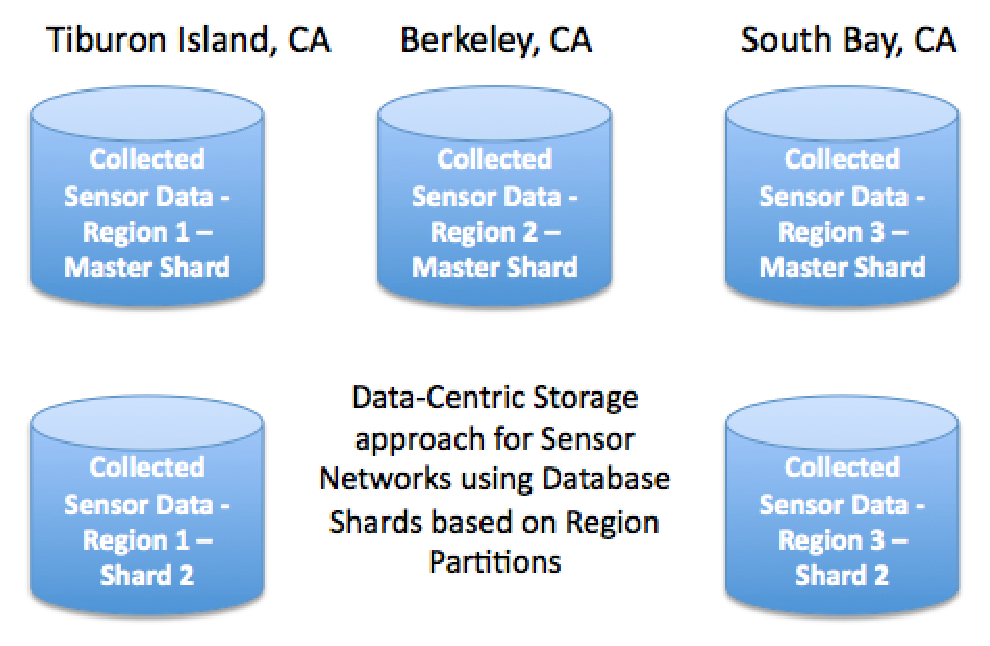
\includegraphics[scale=0.65]{../diagrams/database-sharding-by-region}
  \caption{Example of Data-Centric Storage for Sensor Networks using Database
  Sharding}
  \label{fig:database-sharding-by-region}
\end{figure}

\subsection{Disadvantages of the Data-Centric Approach}

The data partitioning is a very restricted technology, mostly available to
advanced users of distributed database systems. Despite being a capability
being offered common-off-the-shelf by some popular database systems, this
strategy requires closer database management. Some of the problems related to
this strategy are regarding its execution \cite{db-shard-discussion}:

\begin{itemize}
  \item \textbf{Rebalancing Shards}: If the schema model changes for the
  shards, the strategy of rebalancing must be done. For instance, when one of
  the shards outgrows more than the others. As a consequence, the database
  shards must be rebalanced by transferring data to new locations whenever
  necessary. This technique is starting to appear as COTS implemetations such
  as mongoDB \cite{mongodb} or MySQL \cite{mysql};
  \item \textbf{Referential integrity}: any cross-shard queries can represent
  problems since the application layer is responsible to enforce data
  integrity. Examples include verifying constraints of foreign keys when the
  partition is done using Vertical table partitioning, considering that data
  collections are organized in separate spaces, and physically placed in
  different shard nodes \cite{db-table-partition}.
\end{itemize}

\subsection{Technology Analysis}

\begin{itemize}
  \item \textbf{MySQL}: Supports External or Data-Centric Storage approaches.
  When Data-Centric Storage is used, both vertical and horizontal partitions
  \cite{db-partitioning-relational} can be chosen, using different strategies to
  partition the data;
  \item \textbf{Oracle}: Supports External or Data-Centric Storage
  approaches. Only supports vertical partitioning with the definition
  of different types \cite{db-table-partition};
  \cite{db-partitioning-relational-oracle} when using Data-Centric storage;
  \item \textbf{Berkeley TinyDB}: Only supports the External Storage;
  \item \textbf{MongoDB}: Supports External or Data-Centric Storage.
  Using the latter one, only the horizontal partition approach is available
  using with automatic shards \cite{db-mongo-partition};
  \item \textbf{DB2}: Supports External and Data-Centric storage. Only supports
  vertical table partition \cite{db-db2-partition} for the data-centric storage;
\end{itemize}

All the selected database systems supports the External Storage approach.
However, they all differ with the support to Data-Centric Storage support.

\section{Analysis of the Query Processing Mechanism Taxonomy}

As a direct result from the previous section, the use of \textbf{Centralized Query
Processing} is indicated for NetBEAMS, also given the fact that SF-BEAMS data
goes directly to the single network sink, and therefore, a centralized location
of the data.

\subsection{Advantages of the Centralized Query Processing}

Centralized data management and query processing is simpler than the in-network
query method. Data is verified by a simple database management system without
the risk of data being unavailable, when the data is spread among the network
nodes.

\subsection{Disadvantages of the Centralized Query Processing}

When the Centralized Query processing is used, problems may occur. Depending
on the size of the datasets and the database technology, performance may be a
concern. For example, this approach creates of the so-called Funneling
Affect \cite{sn-storage04}, since the point-of-traffic is concentrated in the
centralized system.

In order to mitigate the problems originated by this query processing
mechanism, techniques such as Data Replication can be used.

\subsection{Technology Analysis}

All the database systems technology support a centralized query system.

\section{Analysis of the Data Model Taxonomy}

One of the most common practices in the area of database system is to use the
relational model to persist data, although the application of the system may
not fit to solve the problem. In fact, the main users of sensor networks may
not hold any expertise in database systems or data modeling, given they come
from different science areas. Taking NetBEAMS as an example, we see a Sensor
Network managed by Marine Biologists without expertise in Data Management,
Modeling systems, and for this reason, one of the requirements of the system is
try the use of schema-less approaches. The \textbf{Key-Value-Pair Data Model}
or the \textbf{Document-Oriented Data Model} seems to be the simplest choices of the
models.

\subsection{Analysis of the Schema-Dependent Models}

Considering the inception of a relational data model \cite{relational-model} and
the use of the YSI Sonde data as the main entity in the system, let Figure 
\ref{fig:Relational-Model-Original} represent a prototype of the relational
model, after passing through the process of normalization
\cite{db-normalization}.

\begin{figure}
  \centering
  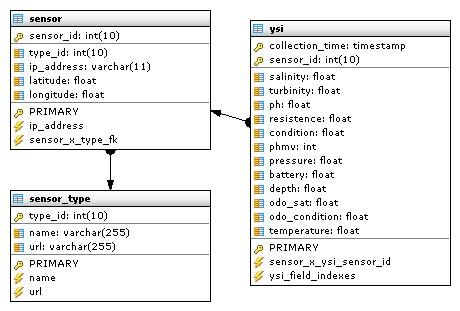
\includegraphics[scale=0.65]{../diagrams/Relational-Model-Original}
  \caption{Relational Data Model for NetBEAMS - A first prototype}
  \label{fig:Relational-Model-Original}
\end{figure}

Supposing a new type is added into the system, let the refactored
version of the relational model be depicted in Figure
\ref{fig:Relational-Model-Addition-Modified}. Some observations are considered
in this scenario:

\begin{figure}
  \centering
  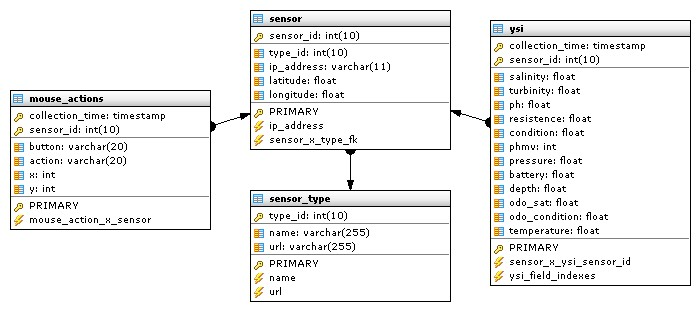
\includegraphics[scale=0.65]{../diagrams/Relational-Model-Addition-Modified}
  \caption{Relational Data Model for NetBEAMS - Modified version with new
  entity}
  \label{fig:Relational-Model-Addition-Modified}
\end{figure}

\begin{itemize}
  \item Constant data schema changes require constant database normalization
  process, changes to structure, database management, etc. Schema-Dependent
  databases always require refactoring of the schema to accommodate changes to
  the entites properties;
  \item The approach of Relational Model might does not fit the nature of
  collected data from wired or wireless sensor networks, since they tend to
  change over time \cite{db-is-rdbs-dommed}. They usually does not give support
  time-series data nor provenance well \cite{sn-provenance};
  \item Some research have suggested changes to the SQL clauses to better
  support time-series \cite{sn-db-newop}.
\end{itemize}

Other projects have been using the XML data models for persistence. It falls
into the same category as the Relational Model using XML documents \cite{xml},
being complaint to an XML Schema \cite{xml-schema}. This model uses XPath
\cite{xml-xpath} technology for querying documents, although some hibrid
technologies may still use SQL \cite{sql} for that matter \cite{db2}. In this
way, a materialized version of the data from the defined previous schema can be
seen in Figure \ref{fig:persistence-example-relational}.

\begin{figure}[!h]
  \centering
  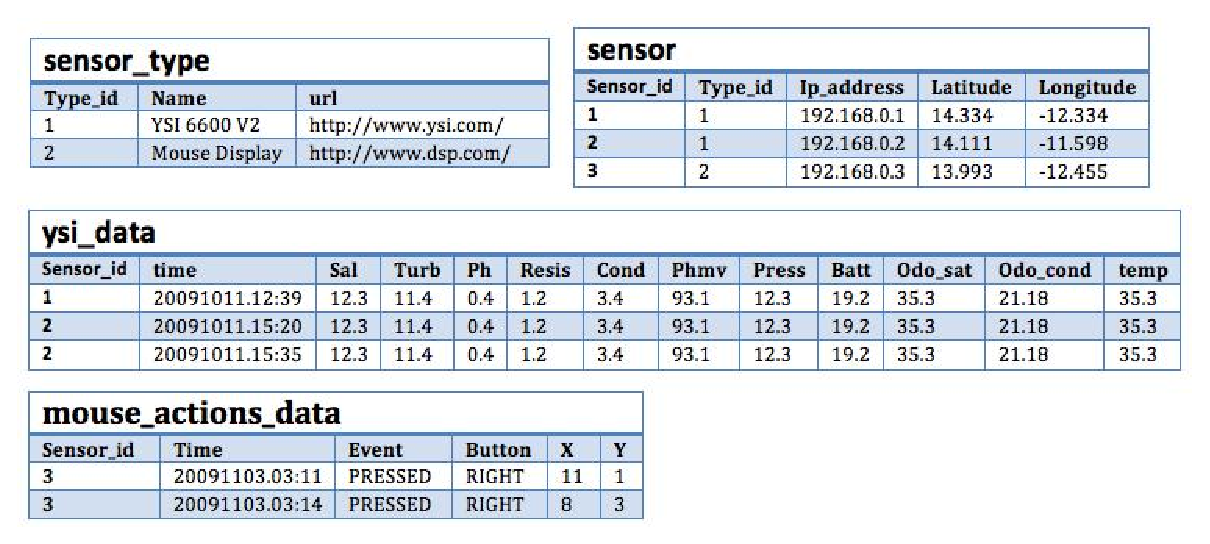
\includegraphics[scale=0.7]{../diagrams/persistence-example-relational}
  \caption{Instance of a Relational Model Database Prototype}
  \label{fig:persistence-example-relational}
\end{figure}

Although this data model have been used in different types of applications,
developers have tried to use the Relational Model to model an application that
could prevent any database change through the use of a technique that relates a
key to a value, called Key-Value data model. With the advent of Internet
applications, the need of such a model that does not need constant refactoring
led developers to propose such approach using the relational model as
documented in technical articles such as \cite{db-kvp-in-relational01} and
\cite{db-kvp-in-relational02}. Based in these articles, consider the relational
model depicted in Figure \ref{fig:KVP-on-Relational-Model} as a data model for
persisting data to our case study using the key-value strategy. The problem
with it is that key repetition occurs, since the nature of time-series data
requires the use of a timestamp key for each property of the sensor. Therefore,
this strategy is not well-suited to provide persistence data from collected
sensor networks.

\begin{figure}[!h]
  \centering
  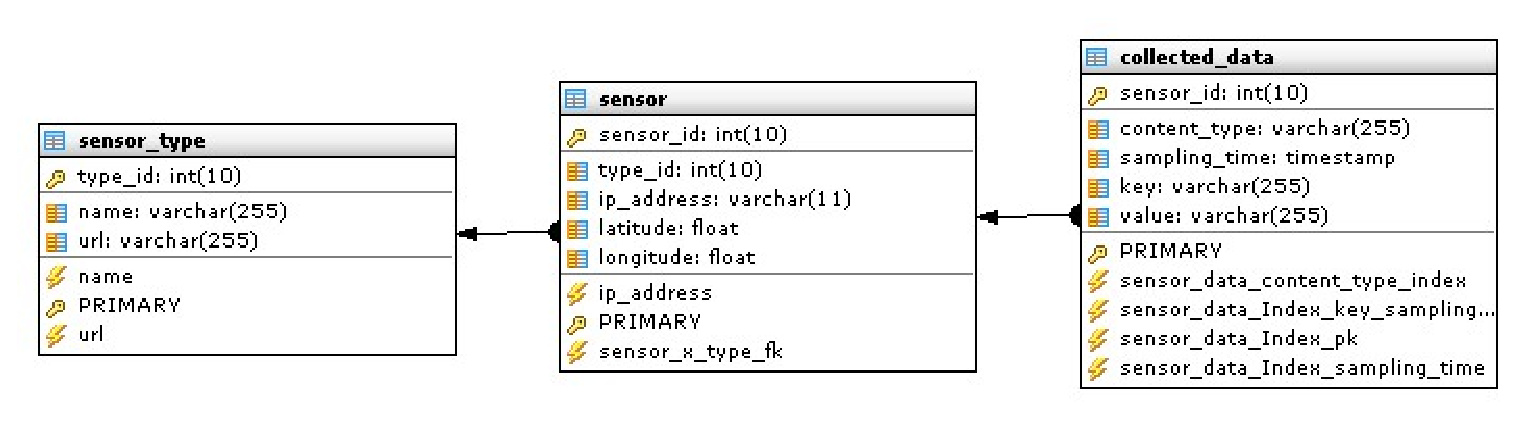
\includegraphics[scale=0.6]{../diagrams/KVP-on-Relational-Model}
  \caption{KVP Data Model implementation using Relational Model}
  \label{fig:KVP-on-Relational-Model}
\end{figure}

\begin{figure}[!h]
  \centering
  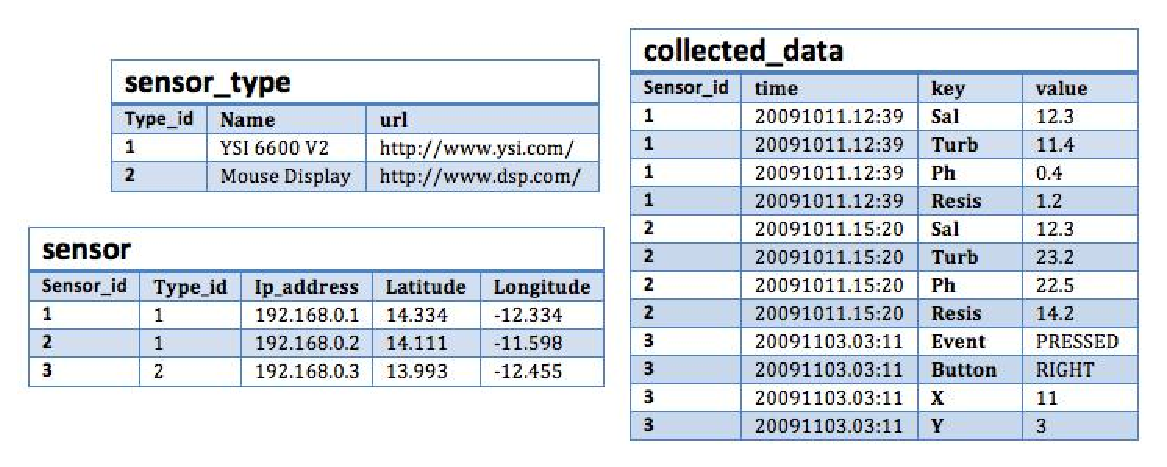
\includegraphics[scale=0.75]{../diagrams/persistence-example-relational-kvp}
  \caption{KVP over Relational Model Database Prototype}
  \label{fig:persistence-example-relational-kvp}
\end{figure}

\subsection{Analysis of the Schema-less Models}

The growth of distributed systems and the Internet have enabled the development
of powerful database servers that can be organized in the context of
infrastructure and how to represent models. An powerful up-coming approach is
the use of database systems that does not use structured language for querying
its data. One such example is called Key-Value Pair (KVP) data model
\cite{db-kvp}, which is also known as Document-Oriented, Distributed Hash
Table. Such a model has the following properties:

\begin{itemize}
  \item data is structured in collections of key-value pairs, as it is done in
  hash data structure. The definition of the key is a given property with its
  associating value;
  \item the query process is using mechanics similar to programming or
  scripting language, that is, the use of APIs in a given programming language.
\end{itemize}

There are no records of the use of this data model with Sensor Networks.
Different variants of such data model is the document-oriented data model,
where data is modeled using structured documents. However, these documents
have a dynamic structure that can be freely described without the use of a
schema validation mechanism as used in XML Schema. One example of such
approach is the use of the JSON data format \cite{json} in the implementation
of database systems which are becoming popular with the new trend called Cloud
Computing \cite{cloud-comp-architectures}. Databases implementing this
strategy is the mongoDB \cite{mongodb}.

\begin{itemize}
  \item entities from the same domains are placed into a ``bucket'';
  \item entities have a set of attributes and relating values
  \item entities with different set of attributes may be contained in the same
  bucket, since there is no schema to govern the bucket items restriction.
\end{itemize}

For instance, all data needed for the YSI sonde data, as well as all necessary
provenance data that describes the data, depicted in section
\ref{sec:sn-provenance}, are represented by means of key-value pairs
\ref{fig:persistence-example-kvp}.

\begin{figure}[!h]
  \centering
  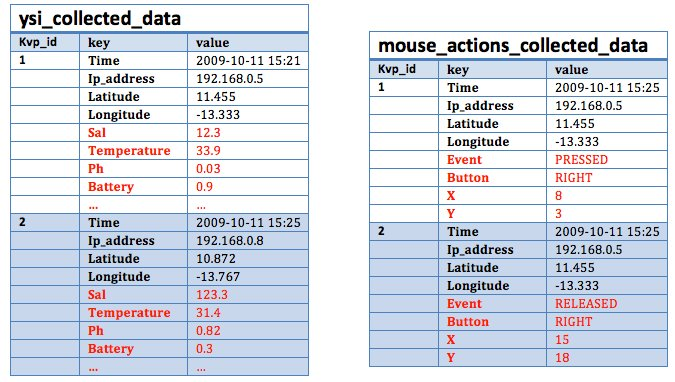
\includegraphics[scale=0.75]{../diagrams/persistence-example-kvp}
  \caption{KVP Database instance Prototype}
  \label{fig:persistence-example-kvp}
\end{figure}

\subsection{Technology Analysis}

The relational and key-value data models were compared by
\cite{db-is-rdbs-dommed} and can be summarized as follows:

\begin{table}
    \label{tab:ysi-data-distribution}
    \caption{Schema-Dependent X Schema-less Databases Compared: Properties}
    \begin{center}
    \begin{tabular}{|p{210pt}|p{210pt}|}\hline
    Schema-Dependent Databases & Schema-less Databases\\\hline
    \begin{enumerate}
      \item Real-world model by entities, classified in tables;
      \item Tables composed by columns and rows. Rows are comprised by column
      values, which have the same schema;
      \item Data Model defined in advance with a schema, which contains
      relationships and constraints to enforce data integrity;
      \item Data represents ``natural'' entities, not application specific;
      \item Data Normalization is the data structuring process to remove data
      duplication, as well as establishing data associations through table
      relationships;
      \item Data Provenance can be provided through data types such as
      ``Timestamp'' for time or float for the GPS float-based coordinates; 
    \end{enumerate} 
    & 
    \begin{enumerate}
      \item Real-world model by entities, classified in Domains;
      \item Domains are similar to tables, but like buckets that contains items
      without a pre-defined schema, what enable them to have different schemas;
      \item Items are identified by keys, as well as have a dynamic set of
      attributes attached to it, however with no schema defined;
      \item Items may represent not only the natural representation of data, but
      also include application-specific data;
      \item Since data may be repeated, no data normalization is done, so that
      integrity is done in the application layer;
      \item Data provenance can be added through the use of keys and relating
      values for the time information and location of the data.
    \end{enumerate}
    \\\hline
    \end{tabular}
    \end{center}
\end{table}

\begin{table}
    \label{tab:ysi-data-distribution}
    \caption{Schema-Dependent X Schema-less Databases: Data Access}
    \begin{center}
    \begin{tabular}{|p{210pt}|p{210pt}|}\hline
    Schema-Dependent Databases & Schema-less Databases\\\hline
    \begin{enumerate}
      \item The basic operations CRUD\footnote{Create-Retrieve-Update-Update
      database operations} data are performed using a structured language such
      as the SQL or XPath;
      \item Query languages can access data from different tables through
      joins, contains functions for aggregation and complex filter.
    \end{enumerate} 
    & 
    \begin{enumerate}
      \item The CRUD operations are performed via API\footnote{Application
      Programming Interface} through programming languages;
      \item Some technologies provide basic SQL-like syntax for filter criteria
      with some predicates like =, !=, <, > that ca be applied;
      \item The data and application integrity logic is placed in the
      application layer.
    \end{enumerate}
    \\\hline
    \end{tabular}
    \end{center}
\end{table}

\begin{table}
    \label{tab:ysi-data-distribution}
    \caption{Schema-Dependent X Schema-less Databases: Application Interface}
    \begin{center}
    \begin{tabular}{|p{210pt}|p{210pt}|}\hline
    Schema-Dependent Databases & Schema-less Databases\\\hline
    \begin{enumerate}
      \item Have their own specific API or through ODBC\footnote{Open Database
      Connectivity};
      \item Data is stored in a format that represents its natural structure,
      and for this reason, in a single or distributed fashion.
    \end{enumerate} 
    & 
    \begin{enumerate}
      \item Systems tend to provide SOAP/REST \cite{http-rest};
      \item \cite{db-is-rdbs-dommed} claims that data is stored in a more
      effective way, requiring only code plumbing for the relational code;
    \end{enumerate}
    \\\hline
    \end{tabular}
    \end{center}
\end{table}

Since the selected data model is the schema-less one, the following can be see
from the technologies:

\begin{itemize}
  \item MySQL: Only supports the Relational Model;
  \item Oracle: Only supports Relational Model;
  \item Berkeley TinyDB: Only supports the Relational Model; 
  \item \textbf{MongoDB}: Supports Document-Oriented Model;
  \item IBM DB2: Only Supports the Relational Model.
\end{itemize}

\section{Analysis of the Database System Organization Taxonomy}

Sensor Network data can be saved in either Centralized or Distributed Systems.
While Centralized Database Systems are easier to manage, it may
face challenges regarding its data. In order to implement a Data-Centric
solution, a distribute database system must be in place in order to manage
the different data by a single node.

\subsection{Advantages of Database Partitioning and Sharding}

\begin{itemize}
  \item Data-Centric queries and data use;
  \item Solves bottleneck problems related to reads/writes;
  \item Decrease the funneling effect by directing queries to given data
  partition;
\end{itemize}

\subsection{Disadvantages of Database Partitioning and Sharding}

\begin{itemize}
  \item Very advanced topics in Database System;
  \item May be easy of use, depending on the application.
\end{itemize}

\subsection{Technology Analysis}

\begin{itemize}
  \item \textbf{MySQL}: Supports Data Replication;
  \item \textbf{Oracle}: Supports Data Replication;
  \item \textbf{Berkeley TinyDB}: NO Supports to distributed data;
  \item \textbf{MongoDB}: Supports Data Replication;
  \item \textbf{IBM DB2}: Supports Data Replication.
\end{itemize}

\section{Other Non-Functional Analysis}

\begin{itemize}
  \item \textbf{Open-source}: Given the fact of the nature of the project, the
  technology to be used must be free of cost \cite{open-source}, that is, no
  costs involved in the adoption of such technology; Together with it is the
  support from the community;
  \item \textbf{Native APIs}: In order to cover the scope of this work defined
  in the previous chapter, the solution for persisting collected sensor data
  must be not only limited to a technology that provides data access, such as
  SQL, but also by other \textbf{data access mechanisms};
  \item \textbf{Hot Backup}: Supports hot backup with less service interruption. 
\end{itemize}

\subsection{Technology Analysis}

Most of the technologies listed provides access to the data sets through the
use of drivers in different programming and scripting languages such as Java,
Python, Perl, etc. Moreover, only TinyDB does not support hot backup.

\begin{itemize}
  \item \textbf{MySQL}: Is open-source, supports hot back and contains
  scripting APIs from the community;
  \item \textbf{Oracle}: It is not Open-Source, but contains lots of support
  from the community. Also APIS are available for the majority of languages;
  \item \textbf{Berkeley TinyDB}: Not open-source;
  \item \textbf{MongoDB}: An open-source database system with an increasing
  support from the community, offering native APIS in different programming
  languages and scripting languages;
  \item \textbf{IBM DB2}: Not Open-Source, but offers support from its
  community.
\end{itemize}

Only MySQL and MongoDB supports the non-functional requirements defined in this
section.

\section{Global Analysis Results and Technology Selection}

Each of the databases were scored according to its support to the different
types of taxonomies, and randomly selected by using the literature review's
list, as well as the Internet. Since mongoDB is based on a schema-less database
system, and supports most of the taxonomies defined in the previous chapter.

\begin{table}
    \label{tab:ysi-data-distribution}
    \caption{Amount of data produced by the RTC's YSI sondes}
        \begin{center}
        \begin{tabular}{|c|c|c|c|c|c|c|}\hline 
        \textbf{Database} & \textbf{MySQL} & \textbf{Oracle} &
        \textbf{TinyDB} & \textbf{MongoDB} & \textbf{IBM DB2}\\\hline 
        Centralized Query & + & + & + & + & + \\\hline 
        Distributed System & ++ & ++ & - & ++ & +\\\hline 
        Schema-less & - & - & - & + & +\\\hline 
        Provenance Support & + & + & + & + & +\\\hline 
        NO-SQL Query & - & - & - & + & +\\\hline 
        Data Partition & + & + & - & + & +\\\hline 
        Hot Backup & + & + & - & - & +\\\hline 
        Export Capability & + & + & - & + & -\\\hline 
        Programming Lang. & + & + & + & + & +\\\hline
        Script Lang. & + & + & - & + & +\\\hline
        Open-Source & + & - & + & + & -\\\hline
        \end{tabular}
        \end{center}
\end{table}